\documentclass[11pt,a4paper]{article}

\usepackage[margin=1in]{geometry}
\usepackage[T1]{fontenc}
\usepackage[utf8]{inputenc}
\usepackage{lmodern}
\usepackage{microtype}
\usepackage{xcolor}
\usepackage{booktabs}
\usepackage{longtable}
\usepackage{array}
\usepackage{enumitem}
\usepackage{hyperref}
\usepackage{listings}
\usepackage{amsmath}
\usepackage{fancyhdr}
\usepackage{float}

\usepackage{tikz}
\usetikzlibrary{arrows.meta,positioning,fit,calc,shapes.geometric,backgrounds}

% Unified Color Palette
\definecolor{navy}{RGB}{28,54,92}
\definecolor{blue2}{RGB}{62,112,170}
\definecolor{lightblue}{RGB}{232,242,252}
\definecolor{green2}{RGB}{50,120,80}
\definecolor{lightgreen}{RGB}{235,247,239}
\definecolor{orange2}{RGB}{190,105,25}
\definecolor{lightorange}{RGB}{252,243,229}
\definecolor{red2}{RGB}{170,55,55}
\definecolor{lightred}{RGB}{252,237,237}
\definecolor{lightgray}{RGB}{245,245,245}
\definecolor{darkgray}{RGB}{80,80,80}

% TikZ Styles
\tikzset{
  agentbox/.style={draw=blue2, rounded corners=4pt, thick,
    minimum width=32mm, minimum height=11mm, align=center, fill=lightblue, font=\small},
  toolbox/.style={draw=green2, rounded corners=4pt, thick,
    minimum width=32mm, minimum height=11mm, align=center, fill=lightgreen, font=\small},
  databox/.style={draw=orange2, rounded corners=4pt, thick,
    minimum width=32mm, minimum height=11mm, align=center, fill=lightorange, font=\small},
  securitybox/.style={draw=red2, rounded corners=4pt, thick,
    minimum width=32mm, minimum height=11mm, align=center, fill=lightred, font=\small},
  flow/.style={-{Latex[length=2mm]}, thick},
  dashedflow/.style={-{Latex[length=2mm]}, thick, dashed},
  decision/.style={diamond, draw=navy, thick, aspect=2, align=center, fill=white, font=\small}
}

\hypersetup{
    colorlinks=true,
    linkcolor=navy,
    urlcolor=navy,
    pdftitle={Multi-Agent Database Analyzer and Agentic Chat Support},
    pdfauthor={Sujeet Banerjee}
}

\pagestyle{fancy}
\fancyhf{}
\lhead{\small Multi-Agent Database Analyzer}
\rhead{\small sujeet.banerjee@gmail.com \\ sujeet.banerjee.professional@gmail.com}
\cfoot{\thepage}

\lstset{
    basicstyle=\ttfamily\small,
    backgroundcolor=\color{lightgray},
    frame=single,
    breaklines=true,
    columns=fullflexible
}

\newcommand{\agent}[1]{\textbf{\textcolor{navy}{#1}}}
\newcommand{\important}[1]{\textbf{#1}}

\title{\textbf{Multi-Agent Database Analyzer}\\
\large Architecture, System Design and Agentic Chat Support}
\author{Sujeet Banerjee}
\date{}

\begin{document}
\maketitle

\begin{abstract}
This paper presents the reference architecture and system design of a multi-agent Database Analyzer that enables users to ask natural-language questions across large-scale enterprise databases and receive evidence-based summaries, root-cause analyses, and conversational insights. The core architectural design principle is that \important{the LLM acts as the planner and interpreter, while the underlying data platform performs heavy computation and serves as the factual evidence base}. The framework incorporates metadata RAG for schema discovery, semantic metric cataloging, self-healing Text-to-SQL generation, deterministic statistical analysis, and strict out-of-band security guardrails.
\end{abstract}

\tableofcontents
\newpage

\section{Problem Statement}

Consider an enterprise analytical environment with databases containing billions of rows covering customers, transactions, orders, support interactions, and operational metrics.

When a user asks:
\begin{quote}
``Summarize our business performance last quarter. Why did revenue decline, and which products and customer segments caused the decline?''
\end{quote}

A naive LLM chatbot cannot ingest raw database tables due to context length limits, extreme token cost, latency, and security risks. Conversely, fixed Text-to-SQL scripts lack multi-step reasoning capabilities to follow up on unexpected anomalies.

An enterprise-grade solution requires an agentic system that acts like a senior data analyst:
\begin{enumerate}[leftmargin=*]
    \item Understands user intent and disambiguates business metrics.
    \item Dynamically discovers relevant schema subsets using Metadata RAG.
    \item Formulates an analytical execution plan.
    \item Generates safe, highly optimized SQL and auto-corrects execution errors.
    \item Pushes heavy aggregations down to the database/OLAP engine.
    \item Applies deterministic statistical checks on returned evidence.
    \item Decides whether additional investigative drill-downs are required.
    \item Synthesizes evidence into clear, auditable explanations with query lineage.
\end{enumerate}

\[
\boxed{\text{Database} \rightarrow \text{LLM} \rightarrow \text{Summary}} \quad \text{\textbf{(Infeasible for Enterprise Scale)}}
\]

\[
\boxed{
\text{User}
\rightarrow
\text{Planner}
\rightarrow
\text{Metadata / Semantics}
\rightarrow
\text{Safe SQL}
\rightarrow
\text{Database}
\rightarrow
\text{Analysis}
\rightarrow
\text{Evidence}
\rightarrow
\text{LLM Summary}
} \quad \text{\textbf{(Target Architecture)}}
\]

\section{System Goals}

\begin{itemize}[leftmargin=*]
    \item \textbf{Natural Language Access:} Seamless chat-based exploration of structured enterprise data.
    \item \textbf{Decoupled Heavy Computation:} Execution remains close to the data platform (Snowflake, BigQuery, Databricks, Postgres).
    \item \textbf{Semantic Precision:} Metric definitions (e.g., Net Revenue) are resolved via a centralized catalog.
    \item \textbf{Bounded Autonomy:} Agentic investigation loops operate under strict budget, latency, and step limits.
    \item \textbf{Defense-in-Depth Security:} RBAC, row-level access control, and PII masking are enforced by the database, not by prompt instructions.
    \item \textbf{Full Traceability:} Every claim in a summary is linked to execution logs, SQL queries, and source tables.
\end{itemize}

\section{Reference Architecture}

Figure~\ref{fig:overview} illustrates the layered reference architecture of the Multi-Agent Database Analyzer.

\begin{figure}[H]
\centering
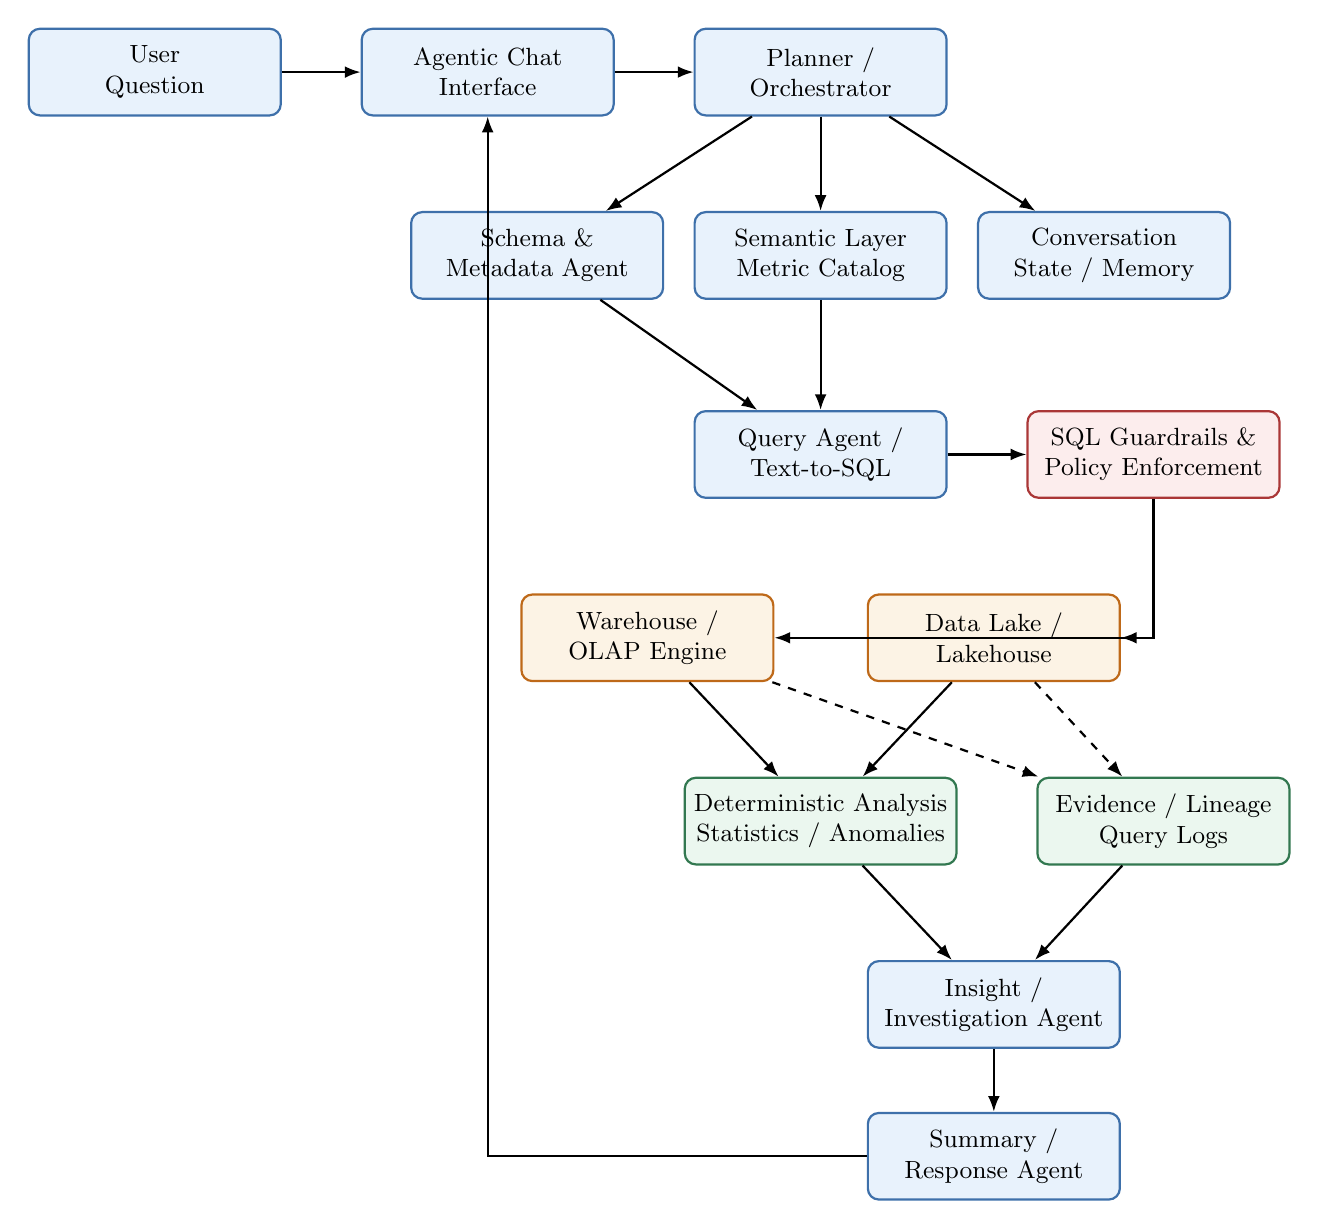
\begin{tikzpicture}[node distance=8mm and 10mm]
% Row 1
\node[agentbox] (user) {User\\Question};
\node[agentbox, right=of user] (chat) {Agentic Chat\\Interface};
\node[agentbox, right=of chat] (planner) {Planner /\\Orchestrator};

% Row 2
\node[agentbox, below=12mm of planner, xshift=-36mm] (schema) {Schema \&\\Metadata Agent};
\node[agentbox, below=12mm of planner] (semantic) {Semantic Layer\\Metric Catalog};
\node[agentbox, below=12mm of planner, xshift=36mm] (memory) {Conversation\\State / Memory};

% Row 3
\node[agentbox, below=14mm of semantic] (query) {Query Agent /\\Text-to-SQL};
\node[securitybox, right=of query] (guard) {SQL Guardrails \&\\Policy Enforcement};

% Row 4
\node[databox, below=12mm of query, xshift=-22mm] (warehouse) {Warehouse /\\OLAP Engine};
\node[databox, below=12mm of query, xshift=22mm] (lake) {Data Lake /\\Lakehouse};

% Row 5
\node[toolbox, below=12mm of warehouse, xshift=22mm] (analysis) {Deterministic Analysis\\Statistics / Anomalies};
\node[toolbox, right=of analysis] (evidence) {Evidence / Lineage\\Query Logs};

% Row 6
\node[agentbox, below=12mm of analysis, xshift=22mm] (insight) {Insight /\\Investigation Agent};
\node[agentbox, below=8mm of insight] (summary) {Summary /\\Response Agent};

% Connections
\draw[flow] (user) -- (chat);
\draw[flow] (chat) -- (planner);
\draw[flow] (planner) -- (schema);
\draw[flow] (planner) -- (semantic);
\draw[flow] (planner) -- (memory);
\draw[flow] (schema) -- (query);
\draw[flow] (semantic) -- (query);
\draw[flow] (query) -- (guard);
\draw[flow] (guard) |- (warehouse);
\draw[flow] (guard) |- (lake);
\draw[flow] (warehouse) -- (analysis);
\draw[flow] (lake) -- (analysis);
\draw[dashedflow] (warehouse) -- (evidence);
\draw[dashedflow] (lake) -- (evidence);
\draw[flow] (analysis) -- (insight);
\draw[flow] (evidence) -- (insight);
\draw[flow] (insight) -- (summary);
\draw[flow] (summary) -| ($(chat.south)+(0,-0.2)$) -- (chat.south);
\end{tikzpicture}
\caption{Layered reference architecture for multi-agent database analysis.}
\label{fig:overview}
\end{figure}

\begin{center}
\fbox{\parbox{0.9\textwidth}{\centering
\textbf{Core Architectural Principle:} The LLM plans and interprets; the data platform performs large-scale computation and provides verifiable evidence.}}
\end{center}

\section{Separation of Agent Responsibilities}

Rather than using a single monolithic prompt, responsibilities are partitioned into specialized functional agents or modular sub-routines.

\begin{figure}[H]
\centering
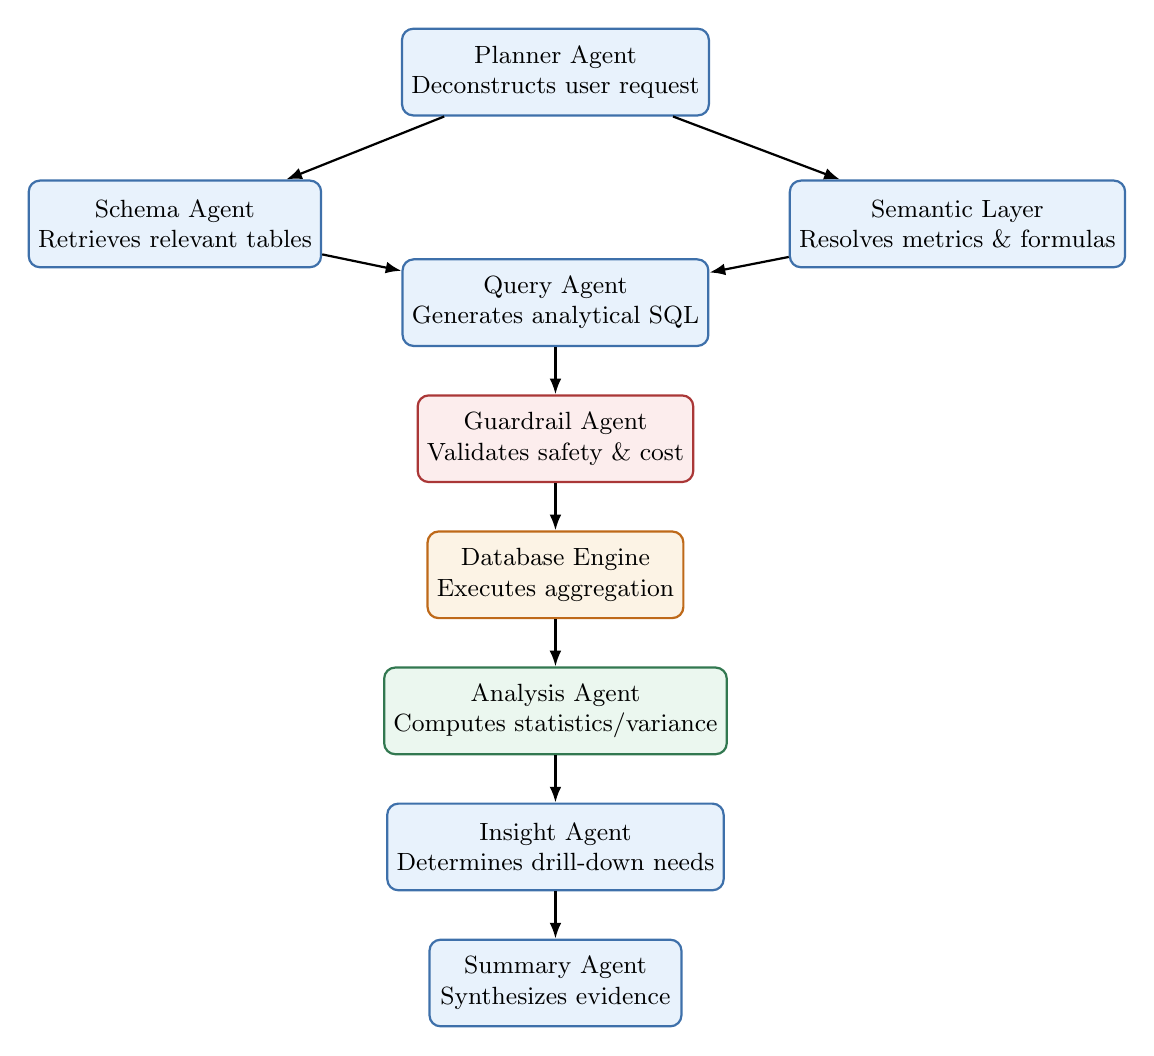
\begin{tikzpicture}[node distance=6mm and 8mm]
\node[agentbox] (p) {Planner Agent\\Deconstructs user request};
\node[agentbox, below left=8mm and 10mm of p] (s) {Schema Agent\\Retrieves relevant tables};
\node[agentbox, below right=8mm and 10mm of p] (m) {Semantic Layer\\Resolves metrics \& formulas};
\node[agentbox, below=18mm of p] (q) {Query Agent\\Generates analytical SQL};
\node[securitybox, below=of q] (g) {Guardrail Agent\\Validates safety \& cost};
\node[databox, below=of g] (d) {Database Engine\\Executes aggregation};
\node[toolbox, below=of d] (a) {Analysis Agent\\Computes statistics/variance};
\node[agentbox, below=of a] (i) {Insight Agent\\Determines drill-down needs};
\node[agentbox, below=of i] (r) {Summary Agent\\Synthesizes evidence};

\draw[flow] (p) -- (s);
\draw[flow] (p) -- (m);
\draw[flow] (s) -- (q);
\draw[flow] (m) -- (q);
\draw[flow] (q) -- (g);
\draw[flow] (g) -- (d);
\draw[flow] (d) -- (a);
\draw[flow] (a) -- (i);
\draw[flow] (i) -- (r);
\end{tikzpicture}
\caption{Modular agent separation of concerns.}
\label{fig:agents}
\end{figure}

\begin{longtable}{p{0.25\textwidth} p{0.68\textwidth}}
\toprule
\textbf{Agent / Module} & \textbf{Primary Responsibility}\\
\midrule
\agent{Planner} & Converts multi-part user prompts into structured analytical plans.\\
\agent{Schema Agent} & Performs hybrid retrieval over metadata catalogs to extract minimal schema details.\\
\agent{Semantic Layer} & Maps business terminology (e.g., ``churn'') to certified database columns and logic.\\
\agent{Query Agent} & Generates dialect-specific analytical SQL with CTEs and window functions.\\
\agent{Guardrail Agent} & Inspects ASTs for safety, syntax correctness, cost ceilings, and RBAC rules.\\
\agent{Analysis Agent} & Executes deterministic statistical tests (variance, trend, anomalies) on aggregate results.\\
\agent{Insight Agent} & Evaluates whether findings satisfy user intent or require further drill-down.\\
\agent{Summary Agent} & Translates verified evidence sets into human-readable narratives with citations.\\
\agent{Memory State} & Maintains conversation history, filter bindings, and entity references.\\
\bottomrule
\end{longtable}

\section{Agentic Investigation Loop \& Self-Healing}

An investigation loop allows the system to drill down autonomously when initial aggregates indicate anomalies (e.g., detecting a regional revenue drop and automatically querying top-affected products).

\begin{figure}[H]
\centering
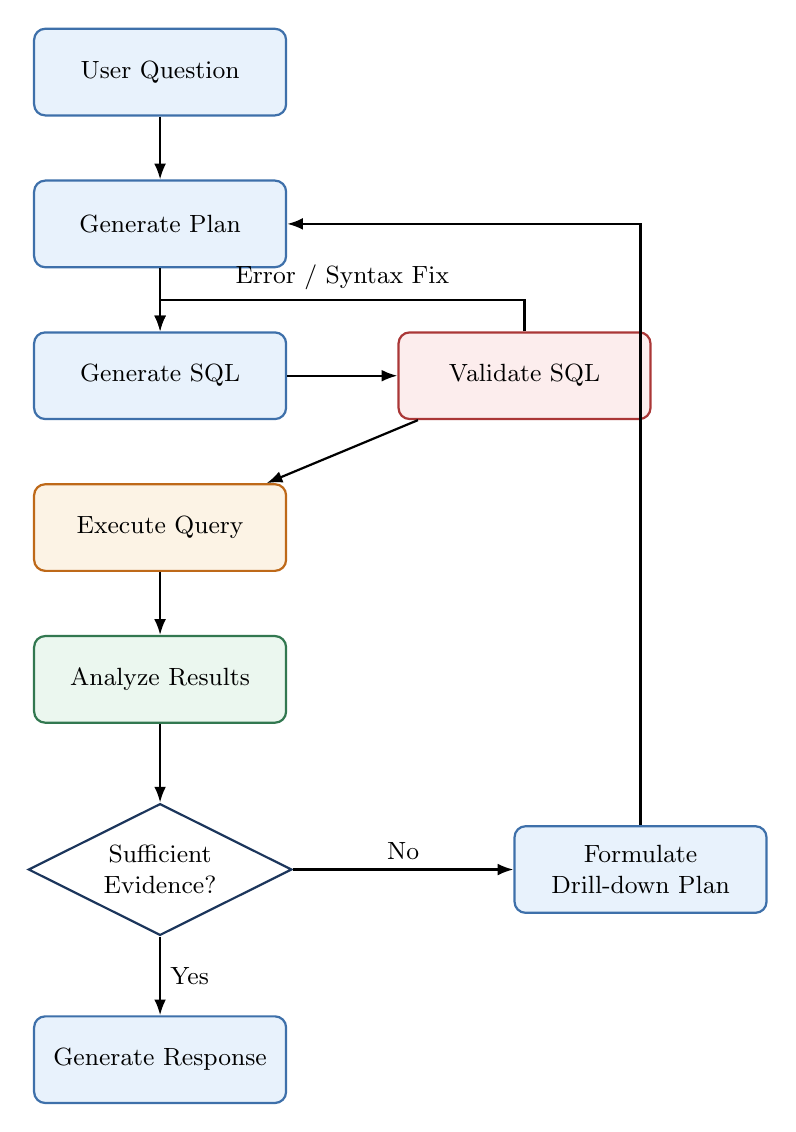
\begin{tikzpicture}[node distance=8mm and 14mm]
\node[agentbox] (q) {User Question};
\node[agentbox, below=of q] (p) {Generate Plan};
\node[agentbox, below=of p] (sql) {Generate SQL};
\node[securitybox, right=of sql] (val) {Validate SQL};
\node[databox, below=of sql] (db) {Execute Query};
\node[toolbox, below=of db] (an) {Analyze Results};
\node[decision, below=10mm of an] (dec) {Sufficient\\Evidence?};
\node[agentbox, below=10mm of dec] (ans) {Generate Response};
\node[agentbox, right=28mm of dec] (drill) {Formulate\\Drill-down Plan};

\draw[flow] (q) -- (p);
\draw[flow] (p) -- (sql);
\draw[flow] (sql) -- (val);
\draw[flow] (val) -- (db);
\draw[flow] (val.north) -- ++(0,0.4) -| node[above, pos=0.25]{\small Error / Syntax Fix} (sql.north);
\draw[flow] (db) -- (an);
\draw[flow] (an) -- (dec);
\draw[flow] (dec) -- node[right]{\small Yes} (ans);
\draw[flow] (dec) -- node[above]{\small No} (drill);
\draw[flow] (drill) |- (p);
\end{tikzpicture}
\caption{Bounded agentic investigation loop with SQL self-healing feedback.}
\label{fig:loop}
\end{figure}

To prevent runaway costs or infinite execution loops, investigation loops must be governed by hard boundaries:
\begin{itemize}
    \item \textbf{Max Iteration Depth:} Limit to a maximum of 3--4 investigation steps per request.
    \item \textbf{Query Budget Ceiling:} Restrict maximum execution time and scanned data quotas per session.
    \item \textbf{Result Set Cap:} Truncate statistical output before sending back to the LLM context.
\end{itemize}

\section{Schema RAG and Semantic Layer}

Supplying an entire corporate database DDL (thousands of tables) to an LLM induces hallucinations and context degradation. The architecture implements \textbf{Metadata RAG} combined with a \textbf{Semantic Layer}.

\begin{figure}[H]
\centering
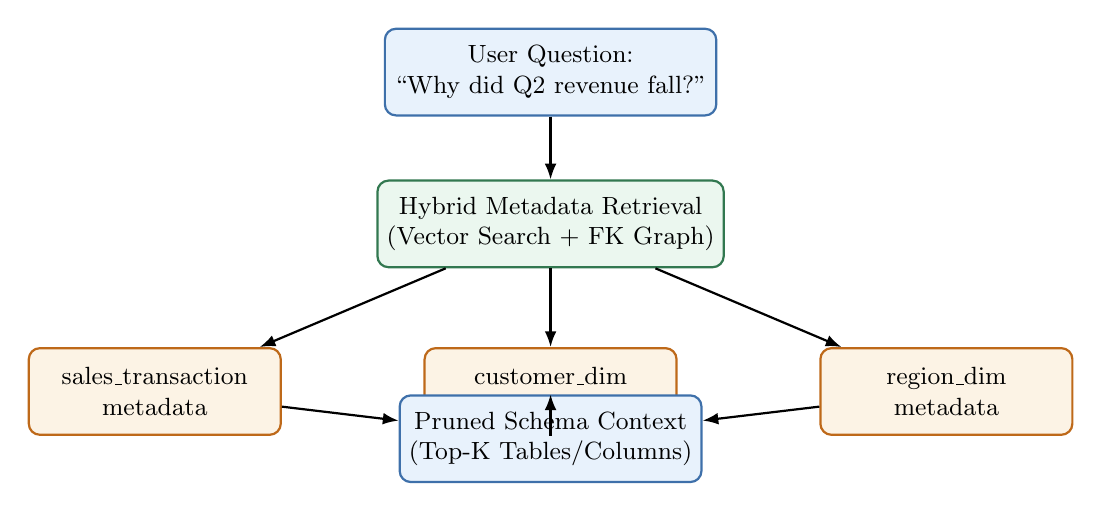
\begin{tikzpicture}[node distance=8mm and 12mm]
\node[agentbox] (question) {User Question:\\``Why did Q2 revenue fall?''};
\node[toolbox, below=of question] (retrieve) {Hybrid Metadata Retrieval\\(Vector Search + FK Graph)};
\node[databox, below left=10mm and 12mm of retrieve] (t1) {sales\_transaction\\metadata};
\node[databox, below=10mm of retrieve] (t2) {customer\_dim\\metadata};
\node[databox, below right=10mm and 12mm of retrieve] (t3) {region\_dim\\metadata};
\node[agentbox, below=16mm of retrieve] (context) {Pruned Schema Context\\(Top-K Tables/Columns)};

\draw[flow] (question) -- (retrieve);
\draw[flow] (retrieve) -- (t1);
\draw[flow] (retrieve) -- (t2);
\draw[flow] (retrieve) -- (t3);
\draw[flow] (t1) -- (context);
\draw[flow] (t2) -- (context);
\draw[flow] (t3) -- (context);
\end{tikzpicture}
\caption{Metadata RAG for dynamically indexing database schemas.}
\label{fig:schemarag}
\end{figure}

The \textbf{Semantic Layer} standardizes complex business logic into verifiable metrics, ensuring that terms like ``Net Revenue'' are calculated consistently.

\begin{figure}[H]
\centering
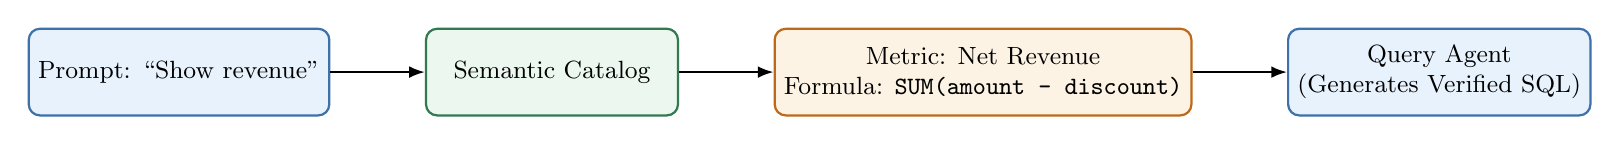
\begin{tikzpicture}[node distance=8mm and 12mm]
\node[agentbox] (q) {Prompt: ``Show revenue''};
\node[toolbox, right=of q] (sem) {Semantic Catalog};
\node[databox, right=of sem] (metric) {Metric: Net Revenue\\Formula: \texttt{SUM(amount - discount)}};
\node[agentbox, right=of metric] (sql) {Query Agent\\(Generates Verified SQL)};

\draw[flow] (q) -- (sem);
\draw[flow] (sem) -- (metric);
\draw[flow] (metric) -- (sql);
\end{tikzpicture}
\caption{Semantic disambiguation preceding query generation.}
\label{fig:semanticlayer}
\end{figure}

\section{Safe Text-to-SQL Execution Path}

To guarantee database safety, query generation must pass through strict validation gates before hitting production engines.

\begin{figure}[H]
\centering
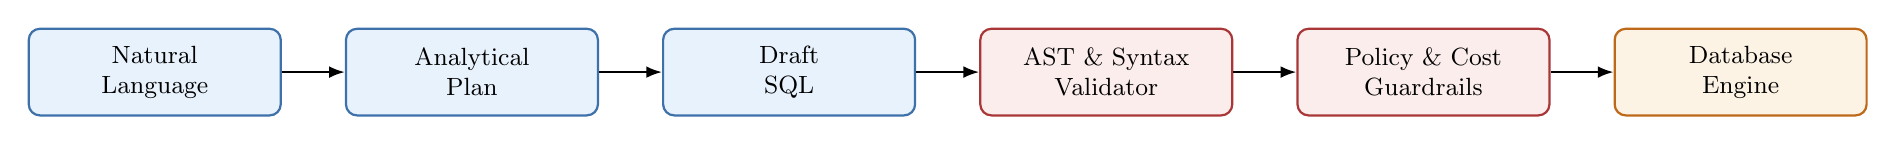
\begin{tikzpicture}[node distance=6mm and 8mm]
\node[agentbox] (nl) {Natural\\Language};
\node[agentbox, right=of nl] (plan) {Analytical\\Plan};
\node[agentbox, right=of plan] (sql) {Draft\\SQL};
\node[securitybox, right=of sql] (v) {AST \& Syntax\\Validator};
\node[securitybox, right=of v] (c) {Policy \& Cost\\Guardrails};
\node[databox, right=of c] (db) {Database\\Engine};

\draw[flow] (nl) -- (plan);
\draw[flow] (plan) -- (sql);
\draw[flow] (sql) -- (v);
\draw[flow] (v) -- (c);
\draw[flow] (c) -- (db);
\end{tikzpicture}
\caption{Safe execution pipeline for generated queries.}
\label{fig:textsql}
\end{figure}

\section{Large-Scale Data Flow & Compute Pushdown}

The architecture guarantees scalability by executing all heavy transformations, joins, and aggregations directly within the database engine.

\begin{figure}[H]
\centering
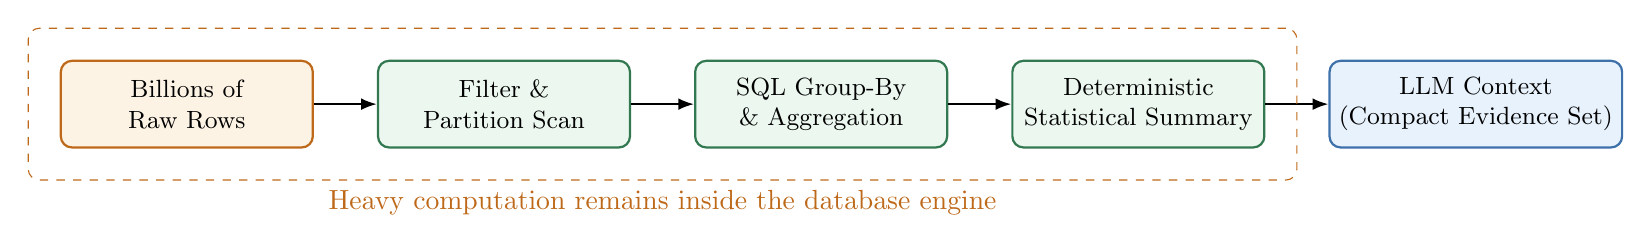
\begin{tikzpicture}[node distance=8mm and 8mm]
\node[databox] (raw) {Billions of\\Raw Rows};
\node[toolbox, right=of raw] (filter) {Filter \&\\Partition Scan};
\node[toolbox, right=of filter] (agg) {SQL Group-By\\\& Aggregation};
\node[toolbox, right=of agg] (stats) {Deterministic\\Statistical Summary};
\node[agentbox, right=of stats] (llm) {LLM Context\\(Compact Evidence Set)};

\draw[flow] (raw) -- (filter);
\draw[flow] (filter) -- (agg);
\draw[flow] (agg) -- (stats);
\draw[flow] (stats) -- (llm);

\node[draw=orange2, dashed, rounded corners, fit=(raw)(filter)(agg)(stats),
      inner sep=4mm, label={[orange2]below:Heavy computation remains inside the database engine}] {};
\end{tikzpicture}
\caption{Compute pushdown pipeline reducing massive raw data to small evidence sets.}
\label{fig:scale}
\end{figure}

\section{Evidence Binding and Lineage}

Every insight presented in the conversational output is bound to specific execution traces. This ensures that conclusions are fully verifiable and auditable.

\begin{figure}[H]
\centering
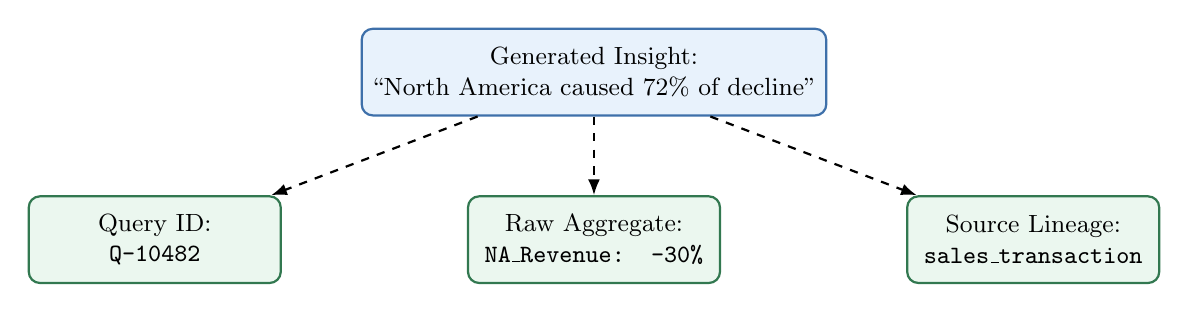
\begin{tikzpicture}[node distance=8mm and 14mm]
\node[agentbox] (insight) {Generated Insight:\\``North America caused 72\% of decline''};
\node[toolbox, below left=10mm and 10mm of insight] (queryid) {Query ID:\\\texttt{Q-10482}};
\node[toolbox, below=10mm of insight] (number) {Raw Aggregate:\\\texttt{NA\_Revenue: -30\%}};
\node[toolbox, below right=10mm and 10mm of insight] (source) {Source Lineage:\\\texttt{sales\_transaction}};

\draw[dashedflow] (insight) -- (queryid);
\draw[dashedflow] (insight) -- (number);
\draw[dashedflow] (insight) -- (source);
\end{tikzpicture}
\caption{Evidence binding architecture for auditability and lineage.}
\label{fig:evidence}
\end{figure}

\section{Defense-in-Depth Security Model}

Security controls must be enforced outside the LLM. The model should never be trusted as an access control mechanism.

\begin{figure}[H]
\centering
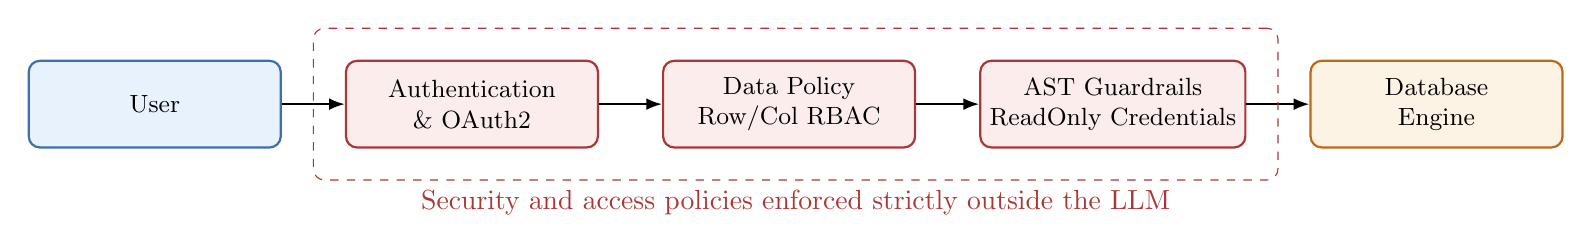
\begin{tikzpicture}[node distance=7mm and 8mm]
\node[agentbox] (user) {User};
\node[securitybox, right=of user] (auth) {Authentication\\\& OAuth2};
\node[securitybox, right=of auth] (policy) {Data Policy\\Row/Col RBAC};
\node[securitybox, right=of policy] (guard) {AST Guardrails\\ReadOnly Credentials};
\node[databox, right=of guard] (db) {Database\\Engine};

\draw[flow] (user) -- (auth);
\draw[flow] (auth) -- (policy);
\draw[flow] (policy) -- (guard);
\draw[flow] (guard) -- (db);

\node[draw=red2, dashed, rounded corners, fit=(auth)(policy)(guard),
      inner sep=4mm, label={[red2]below:Security and access policies enforced strictly outside the LLM}] {};
\end{tikzpicture}
\caption{Out-of-band security and access enforcement model.}
\label{fig:security}
\end{figure}

\section{System Bottlenecks & Mitigations}

\begin{longtable}{p{0.20\textwidth} p{0.32\textwidth} p{0.38\textwidth}}
\toprule
\textbf{Bottleneck} & \textbf{Risk / Impact} & \textbf{Architectural Mitigation}\\
\midrule
Context Overflow & Massive DDLs exceed LLM context window. & Metadata RAG and top-K column indexing.\\
Expensive Scans & Poorly constructed queries lock database tables. & Query cost estimators, timeouts, and required partitions.\\
Metric Confusion & LLM hallucinating metric formulas. & Centralized Semantic Layer / Metric Catalog.\\
Loop Explosion & Infinite agentic investigation loops. & Bounded iteration steps and query budget limits.\\
Security Violations & Prompt injection attempting data exfiltration. & Out-of-band database RBAC and read-only connections.\\
\bottomrule
\end{longtable}

\section{Recommended Proof-of-Concept (POC) Roadmap}

A phased roadmap for implementing a production-grade database analyzer:

\begin{figure}[H]
\centering
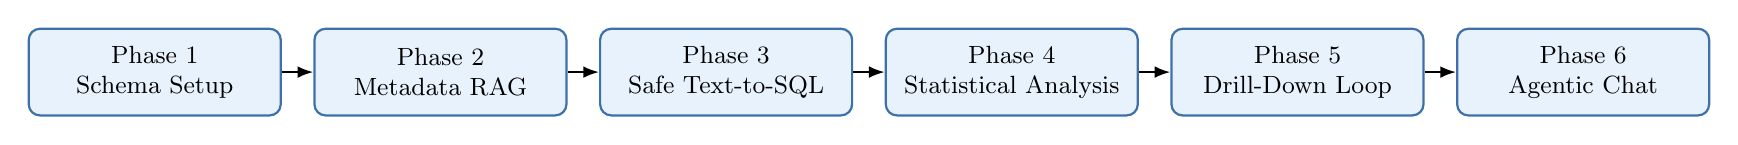
\begin{tikzpicture}[node distance=4mm and 4mm]
\node[agentbox] (p1) {Phase 1\\Schema Setup};
\node[agentbox, right=of p1] (p2) {Phase 2\\Metadata RAG};
\node[agentbox, right=of p2] (p3) {Phase 3\\Safe Text-to-SQL};
\node[agentbox, right=of p3] (p4) {Phase 4\\Statistical Analysis};
\node[agentbox, right=of p4] (p5) {Phase 5\\Drill-Down Loop};
\node[agentbox, right=of p5] (p6) {Phase 6\\Agentic Chat};

\draw[flow] (p1) -- (p2);
\draw[flow] (p2) -- (p3);
\draw[flow] (p3) -- (p4);
\draw[flow] (p4) -- (p5);
\draw[flow] (p5) -- (p6);
\end{tikzpicture}
\caption{Incremental POC development roadmap.}
\label{fig:roadmap}
\end{figure}

\section{Key Architectural Takeaway}

\begin{center}
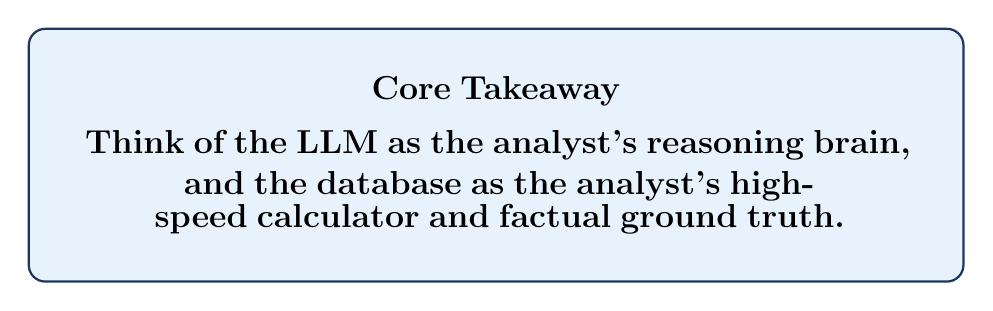
\begin{tikzpicture}
\node[draw=navy, rounded corners=6pt, thick, fill=lightblue,
      text width=0.88\textwidth, align=center, inner sep=6mm] {
\large \textbf{Core Takeaway}\\[2mm]
\textbf{Think of the LLM as the analyst's reasoning brain,}\\[1mm]
\textbf{and the database as the analyst's high-speed calculator and factual ground truth.}
};
\end{tikzpicture}
\end{center}

\end{document}